\documentclass[12pt,a4paper]{article}

\usepackage[spanish]{babel}
\usepackage[utf8]{inputenc}
\usepackage[T1]{fontenc}
\usepackage{lmodern}
\usepackage[a4paper,margin=2.5cm]{geometry}
\usepackage{setspace}
\usepackage{amsmath,amssymb,amsthm}
\usepackage{booktabs}
\usepackage{longtable}
\usepackage{array}
\usepackage{enumitem}
\usepackage{hyperref}
\usepackage{float}
\usepackage{listings}
\usepackage{xcolor}
\usepackage{caption}
\usepackage{graphicx}
\usepackage{fancyhdr}

\pagestyle{fancy}
\fancyhf{}
\lhead{Facultad de Informática de Barcelona}
\rhead{Red de sensorización - OPT}
\cfoot{\thepage}

\hypersetup{
    colorlinks=true,
    linkcolor=black,
    urlcolor=blue,
    citecolor=black,
    pdftitle={Práctica 2 - Diseño de la red de sensorización},
    pdfauthor={Jan Estrada, Adrian nsq}
}

\setstretch{1.15}
\setlength{\parskip}{0.5em}
\setlength{\parindent}{0pt}

\definecolor{codegray}{rgb}{0.95,0.95,0.95}
\definecolor{codecomment}{rgb}{0.2,0.45,0.2}
\definecolor{codekeyword}{rgb}{0.1,0.1,0.6}

\lstdefinelanguage{ampl}{
    morekeywords={set,param,var,maximize,minimize,subject,to,sum,within,binary,integer},
    sensitive=true,
    morecomment=[l]{\#},
    morestring=[b]"
}

\lstset{
    basicstyle=\ttfamily\small,
    backgroundcolor=\color{codegray},
    frame=single,
    breaklines=true,
    showstringspaces=false,
    commentstyle=\color{codecomment},
    keywordstyle=\color{codekeyword},
    columns=fullflexible
}

\begin{document}

\begin{titlepage}
    \centering
    {\Large \textbf{Optimización}}\\[0.3cm]
    {\large GIA UPC}\\[1cm]

    {\huge \textbf{Práctica 2}}\\[0.3cm]
    {\Large Diseño de la red de sensorización para l'Eixample de Barcelona}\\[1.3cm]


    \begin{figure}[H]
        \centering
        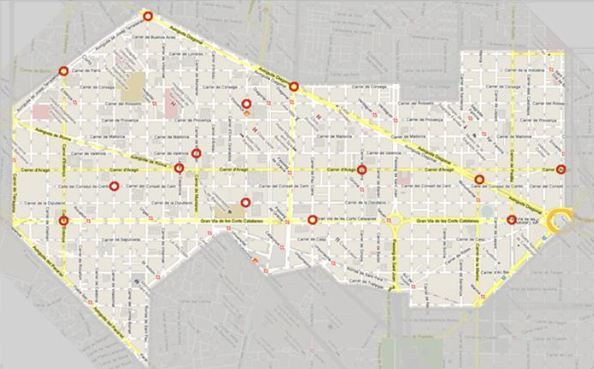
\includegraphics[width=1\linewidth]{image.png}
        \caption{Mapa de la zona de estudio en l'Eixample de Barcelona.}
        \label{fig:eixample}
    \end{figure}



    \textbf{Autores}\\[0.3cm]
    Jan Estrada --- DNI:  \texttt{26314272H}\\
    Adrian Martínez --- DNI: \texttt{49217059A}\\[1.2cm]

    \textbf{Fecha}\\
    Marzo de 2026\\[2cm]


    \vfill
    

\end{titlepage}

\tableofcontents
\newpage

\section{Introducción}

En esta práctica se aborda un problema de localización de sensores en una red urbana de intersecciones. El objetivo es determinar en qué puntos conviene instalar los sensores para maximizar el flujo de vehículos detectado, respetando las restricciones planteadas en el enunciado.

Para ello, se han formulado dos modelos de programación lineal entera. Además de la formulación matemática, en el trabajo también se describe el tratamiento previo de los datos, la implementación en AMPL y el análisis de las soluciones obtenidas.

\subsection{Descripción del problema}

Se dispone de un conjunto de intersecciones y de una colección de caminos de la red, cada uno con un flujo asociado. Un camino se considera detectado cuando al menos dos de sus intersecciones tienen sensor, y el objetivo consiste en maximizar la suma de los flujos de los caminos detectados.

El problema incluye además varias restricciones. Por una parte, solo pueden instalarse como máximo 15 sensores y existen intersecciones fijas y prohibidas. Por otra, en el apartado B se añade la condición de que no puede haber dos sensores situados en intersecciones vecinas, es decir, a una distancia menor o igual a 300 metros.

Concretamente, la red sobre la que trabajamos en este problema está compuesta por 457 intersecciones y 42 caminos a detectar. Las posibles ubicaciones para considerar un camino como válido son 542 pares ruta-intersección, y, para evaluar las distancias de separación del apartado B, contamos con 1284 pares de intersecciones vecinas.
\subsection{Estructura de la entrega}

La entrega se organiza en dos carpetas y el presente documento. En la carpeta \texttt{ampl/} se incluyen los modelos \texttt{practica2\_a.mod} y \texttt{practica2\_b.mod}, los archivos de ejecución \texttt{practica2\_a.run} y \texttt{practica2\_b.run}, y el fichero de datos \texttt{practica2.dat}, compartido por ambos apartados. La carpeta \texttt{tools/} contiene los scripts auxiliares en Python empleados para generar el fichero \texttt{.dat} a partir de los datos crudos y para verificar la consistencia de los datos antes de la ejecución. Finalmente, se adjunta el documento \texttt{informe\_practica2.pdf}, que recoge la formulación, la implementación y el análisis de resultados.

\section{Formulación matemática}

\subsection{Apartado A}

\subsubsection{Conjuntos}

Definimos los siguientes conjuntos:

\begin{itemize}
    \item \(I\): conjunto de todas las intersecciones.
    \item \(P\): conjunto de todos los caminos.
    \item \(F \subseteq I\): conjunto de intersecciones fijas.
    \item \(Q \subseteq I\): conjunto de intersecciones prohibidas.
    \item \(I_p \subseteq I\): conjunto de intersecciones que pertenecen al camino \(p \in P\).
\end{itemize}

\subsubsection{Parámetros}

\begin{itemize}
    \item \(f_p > 0\): flujo asociado al camino \(p \in P\).
\end{itemize}

El flujo se declara como estrictamente positivo (\(f_p > 0\)) y no simplemente como no negativo (\(f_p \geq 0\)) porque todos los valores proporcionados en los datos del enunciado son mayores que cero. Esta condición es relevante para la formulación, ya que garantiza que al solver siempre le convenga activar \(y_p\) cuando el camino disponga de suficientes sensores, y por tanto no sea necesaria una restricción adicional que fuerce \(y_p = 1\).

\subsubsection{Variables de decisión}

\begin{itemize}
    \item \(x_i \in \{0,1\}\), para todo \(i \in I\): vale 1 si se instala un sensor en la intersección \(i\).
    \item \(y_p \in \{0,1\}\), para todo \(p \in P\): vale 1 si el camino \(p\) se considera detectado.
\end{itemize}

\subsubsection{Función objetivo}

Se desea maximizar el flujo total detectado:

\[
\max Z = \sum_{p \in P} f_p \, y_p
\]

\subsubsection{Restricciones}

\begin{align*}
\sum_{i \in I} x_i &\leq 15 && \text{(límite máximo de sensores)} \\
x_i &= 1 \quad \forall i \in F && \text{(intersecciones fijas)} \\
x_i &= 0 \quad \forall i \in Q && \text{(intersecciones prohibidas)} \\
\sum_{i \in I_p} x_i &\geq 2y_p \quad \forall p \in P && \text{(detección de caminos)}
\end{align*}



La última restricción asegura que un camino solo se considere detectado si tiene al menos dos intersecciones con sensor. No hace falta añadir otra restricción para imponer \(y_p = 1\), porque, como todos los flujos son positivos y la función objetivo se maximiza, al solver siempre le interesa activar \(y_p\) cuando puede hacerlo.

\subsection{Apartado B}

El apartado B reutiliza la formulación anterior e incorpora una restricción técnica adicional: dos sensores no pueden situarse simultáneamente en intersecciones vecinas, es decir, a una distancia menor o igual que 300 metros.

\subsubsection{Conjunto adicional}

\begin{itemize}
    \item \(N \subseteq I \times I\): conjunto de pares de intersecciones vecinas.
\end{itemize}

En la implementación, este conjunto se construye normalizando cada par como \((\min(i,j), \max(i,j))\), para evitar duplicados simétricos y no generar dos veces la misma restricción.

\subsubsection{Restricción adicional}

\[
x_i + x_j \leq 1 \quad \forall (i,j) \in N
\]

Esta restricción impide que dos sensores queden demasiado próximos y hace el modelo más restrictivo que en el apartado A. Como consecuencia, la solución óptima del apartado B no puede mejorar la del apartado A en valor de flujo detectado, ya que se obtiene sobre un conjunto factible más pequeño.

\section{Scripts de Python}

\subsection{Uso de los scripts}

Como el fichero original de la práctica estaba en formato \texttt{.txt} y no podía utilizarse directamente en AMPL, se emplearon dos scripts auxiliares en Python. Su función no forma parte del modelo matemático en sí, pero sí del preprocesado necesario para trabajar con los datos.

El primero genera automáticamente el fichero \texttt{practica2.dat} a partir del archivo crudo, mientras que el segundo realiza una comprobación previa sobre los nodos fijos y sus vecindades. De este modo, antes de ejecutar los modelos en AMPL, se puede verificar que los datos están bien estructurados y que no existe ninguna incompatibilidad evidente en el apartado B.

\subsection{Generación del fichero \texttt{.dat}}

El script \texttt{build\_ampl\_data.py} lee el fichero original por secciones y construye a partir de él el archivo \texttt{practica2.dat}, ya en el formato requerido por AMPL. En concreto, extrae los conjuntos \texttt{INTERSECTIONS}, \texttt{PATHS}, \texttt{FIXED} y \texttt{PROHIBITED}, copia los valores de \texttt{PATH\_FLOW}, construye el conjunto \texttt{PATH\_INTERSECTIONS} como pares \texttt{(camino, intersección)} y genera también el conjunto \texttt{NEIGHBORS}.

En el caso de las vecindades, cada par se normaliza como \((\min(i,j), \max(i,j))\) y se descarta cualquier par reflexivo, es decir, aquellos en los que ambos nodos coinciden. De este modo se guarda cada vecindad una sola vez y se evita que el modelo del apartado B genere restricciones duplicadas o triviales.

Se ha optado por generar un único fichero \texttt{.dat} compartido por los dos apartados para facilitar la visualización y evitar repetir código y duplicar archivos. Por este motivo, el fichero incluye también el conjunto \texttt{NEIGHBORS}, que solo es necesario para el apartado B. Como consecuencia, el modelo del apartado A debe declarar este conjunto aunque no lo utilice en ninguna restricción, de modo que AMPL pueda leer el fichero sin generar errores por conjuntos no definidos. Para nuestro caso y modelo no supone ningún problema, ya que el conjunto está vacío y el sobrecoste computacional es despreciable.



\subsection{Verificación de nodos fijos}

El segundo script, \texttt{verify\_fixed\_intersections.py}, se utiliza como comprobación adicional antes de resolver el apartado B. Su objetivo es comprobar de forma explícita si existen dos nodos del conjunto \texttt{FIXED} que además sean vecinos entre sí. Si eso ocurriera, el modelo sería infactible desde el inicio, ya que esos sensores serían simultáneamente obligatorios y prohibidos de coexistir por la restricción de proximidad.

Tras ejecutar el script, se verificó que ninguno de los ocho nodos fijos (\texttt{30}, \texttt{78}, \texttt{44628}, \texttt{45173}, \texttt{45481}, \texttt{45555}, \texttt{45787} y \texttt{49180}) tiene como vecino a otro nodo fijo. Por tanto, el apartado B puede resolverse con normalidad y no presenta una infactibilidad estructural previa debida a los datos. Esta comprobación es importante porque, de existir dicho conflicto, el solver devolvería un problema infactible sin que quedara claro si la causa es la restricción de vecindad o un error en los datos.


\section{Implementación en AMPL}

\subsection{Modelo del apartado A}

La implementación del apartado A en AMPL se ha mantenido muy próxima a la formulación matemática. Se declaran los conjuntos \texttt{INTERSECTIONS}, \texttt{PATHS}, \texttt{FIXED}, \texttt{PROHIBITED} y \texttt{PATH\_INTERSECTIONS}, junto con el parámetro \texttt{PATH\_FLOW} y las variables binarias \texttt{x} e \texttt{y}.

Cabe destacar una diferencia de modelado entre la formulación matemática y la implementación en AMPL. En la formulación se define \(I_p \subseteq I\) como el subconjunto de intersecciones del camino \(p\), y la restricción de detección se escribe como \(\sum_{i \in I_p} x_i \geq 2y_p\). En AMPL, esta familia de subconjuntos se implementa de forma equivalente mediante un único conjunto bidimensional \texttt{PATH\_INTERSECTIONS} \(\subseteq P \times I\), donde el par \texttt{(p, i)} pertenece al conjunto si la intersección \texttt{i} forma parte del camino \texttt{p}. Ambas representaciones son equivalentes, pero la segunda permite una sintaxis más compacta en AMPL.

La función objetivo maximiza el flujo total detectado, y las restricciones reproducen exactamente el número de sensores máximo, la detección de caminos y la activación o prohibición de sensores en intersecciones concretas. Además, en este modelo se declara también el conjunto \texttt{NEIGHBORS}, aunque no interviene en ninguna restricción del apartado A, tal y como se ha comentado anteriormente.

En lugar de detallar el código fuente completo, que se adjunta en la carpeta \texttt{ampl/}, cabe destacar la formulación de la restricción clave de detección de caminos. En AMPL, aprovechando el conjunto bidimensional \texttt{PATH\_INTERSECTIONS}, esta restricción se escribe de la siguiente forma compacta:

\begin{lstlisting}[language=ampl]
subject to detected_paths {p in PATHS}:
    sum {(p, i) in PATH_INTERSECTIONS} x[i] >= 2 * y[p];
\end{lstlisting}

Las demás restricciones se codifican mediante igualdades directas o sumatorios sencillos sobre el conjunto de intersecciones.

\subsection{Modelo del apartado B}

El modelo del apartado B es idéntico al del apartado A, salvo por la incorporación de la restricción adicional de separación. Esta restricción utiliza el conjunto \texttt{NEIGHBORS} y se implementa evitando que la suma de los sensores en dos intersecciones vecinas supere el valor 1:

\begin{lstlisting}[language=ampl]
subject to separated_sensors {(i, j) in NEIGHBORS}:
    x[i] + x[j] <= 1;
\end{lstlisting}

El resto del modelo y de la función objetivo son idénticos respecto a la base del apartado A.

\subsection{Archivos de ejecución}

Para cada apartado se ha creado un fichero \texttt{.run} que automatiza el flujo de trabajo en AMPL: cargar el modelo, leer los datos, seleccionar el solver, resolver el problema y mostrar los resultados. A modo de ejemplo, el fichero \texttt{practica2\_a.run} contiene las instrucciones siguientes:

\begin{lstlisting}[language=ampl,caption={Fichero de ejecución del apartado A}]
model practica2_a.mod;
data practica2.dat;
option solver gurobi;
solve;
display total_flow;
display {i in INTERSECTIONS : x[i] = 1} x[i];
display {p in PATHS : y[p] = 1} y[p];
\end{lstlisting}

La instrucción \texttt{display} filtra las variables con valor 1 para mostrar únicamente los sensores seleccionados y los caminos detectados, lo que facilita la lectura de los resultados y su incorporación directa al análisis.

En cuanto al solver, se ha utilizado Gurobi 12.0.3 en ambos apartados. Inicialmente se valoró la posibilidad de recurrir al servidor NEOS para la resolución, dado que la licencia académica de AMPL puede imponer límites en el número de variables. Sin embargo, el modelo tiene un tamaño moderado 499 variables binarias (457 para \texttt{x} y 42 para \texttt{y}) y un número de restricciones contenido y se pudo resolver de forma local con los solvers disponibles en dicha licencia de AMPL.

\section{Resultados}

\subsection{Resumen general}

Ambos apartados se resolvieron a optimalidad utilizando el solver Gurobi. En los dos casos, el modelo instaló el máximo permitido de 15 sensores y logró detectar con éxito 24 caminos de la red. 

En cuanto a la función objetivo, el apartado A alcanza un flujo total detectado de 350.7337301, mientras que en el apartado B el valor óptimo es ligeramente inferior, situándose en 350.1781172. 

\subsection{Sensores seleccionados}

Las intersecciones activadas por la solución óptima del apartado A son las siguientes:

\begin{table}[H]
\centering
\caption{Intersecciones con sensor en la solución del apartado A}
\begin{tabular}{ccccc}
\toprule
\multicolumn{5}{c}{\textbf{Nodos seleccionados}} \\
\midrule
5 & 30 & 78 & 20349 & 41633 \\
41970 & 44494 & 44604 & 44628 & 45173 \\
45481 & 45555 & 45787 & 49180 & 54839 \\
\bottomrule
\end{tabular}
\end{table}

En el apartado B, la solución óptima cambia algunos nodos para respetar la restricción de separación entre intersecciones vecinas:

\begin{table}[H]
\centering
\caption{Intersecciones con sensor en la solución del apartado B}
\begin{tabular}{ccccc}
\toprule
\multicolumn{5}{c}{\textbf{Nodos seleccionados}} \\
\midrule
5 & 30 & 78 & 41633 & 41653 \\
41970 & 44522 & 44609 & 44628 & 45173 \\
45481 & 45555 & 45787 & 49180 & 54839 \\
\bottomrule
\end{tabular}
\end{table}

\subsection{Interpretación de resultados}

El apartado A proporciona la mejor solución posible cuando solo se consideran las restricciones básicas del problema. En este caso, el modelo selecciona los 15 sensores disponibles y consigue detectar 24 caminos, alcanzando el mayor flujo total de los dos apartados.

En el apartado B también se instalan 15 sensores y se detectan 24 caminos, pero el flujo total baja ligeramente. Esto se debe a que la restricción de separación obliga a sustituir algunas intersecciones de la solución del apartado A por otras alternativas, lo que reduce ligeramente la calidad final de la solución. En concreto, desaparecen los nodos 20349, 44494 y 44604, y pasan a seleccionarse 41653, 44522 y 44609.

Analizando los datos de vecindad se puede identificar el motivo de cada sustitución. Los nodos 5 y 44494 aparecen como vecinos en el conjunto \texttt{NEIGHBORS}, por lo que no pueden estar activos a la vez en el apartado B. Del mismo modo, los nodos 20349 y 41633 también son vecinos. En ambos casos, el solver se ve obligado a elegir solo uno de los dos nodos de cada par conflictivo. Por otro lado, el nodo 44604 es vecino de 44609, con lo cual el solver no puede seleccionar simultáneamente ambos y opta por 44609 en su lugar. En definitiva, las sustituciones que realiza el modelo en el apartado B son consecuencia directa de la restricción de proximidad.

La diferencia entre ambos valores óptimos es pequeña, de 0.5556129 unidades de flujo. Esto indica que la restricción adicional del apartado B afecta a la solución, pero no perjudica gravemente el flujo total captado.

\section{Discusión de la implementación y conclusiones}

La resolución de la práctica se ha basado en una formulación entera lineal clara y en una implementación sencilla en AMPL, apoyada por un preprocesado previo en Python para convertir el fichero \texttt{.txt} al formato \texttt{.dat}. Esta parte previa ha sido útil para trabajar con los datos de forma ordenada, evitar errores manuales y comprobar que el conjunto de información utilizado por el modelo era consistente antes de ejecutar los solvers.

En conjunto, los resultados obtenidos muestran que el modelo representa correctamente las condiciones del problema en los apartados A y B. No obstante, en una aplicación real sería imprescindible asegurar que las restricciones técnicas se cumplen exactamente como se han modelado, especialmente en el caso de la distancia mínima entre sensores. Si en la instalación real un sensor se colocara ligeramente más cerca de lo permitido por un error de medida, una limitación física o un problema de ejecución, la validez de la solución podría verse afectada y el comportamiento de la red cambiar de forma importante.


\section*{Bibliografía}
\begin{itemize}
    \item Universitat Politècnica de Catalunya. Enunciado de proyecto: \textit{Práctica 2 - Diseño de una red de sensorización}. 
    \item Universitat Politècnica de Catalunya. Apuntes de teoría y laboratorio: \textit{OPT\_T5 - Programación Lineal entera} y recursos de \textit{AMPL - A Mathematical Programming Language}. 
    \item Contribuidores de Wikipedia. \textit{Maximum coverage problem}, \textit{Set cover problem} e \textit{Integer programming}. Wikipedia, The Free Encyclopedia. \url{https://en.wikipedia.org/wiki/Maximum_coverage_problem}, \url{https://en.wikipedia.org/wiki/Set_cover_problem}, \url{https://en.wikipedia.org/wiki/Integer_programming}.
    \item Mehr, N. \& Horowitz, R. (2018). \textit{A Submodular Approach for Optimal Sensor Placement in Traffic Networks}. American Control Conference (ACC). \url{https://horowitz.me.berkeley.edu/Publications_files/All_papers_numbered/Mehr_Submodular_Optimal_Sensor_Placement_ACC2018.pdf}
    \item Kaiser, S. K. (2026). \textit{Sensor Placement for Urban Traffic Interpolation: A Data-Driven Evaluation to Inform Policy}. arXiv preprint arXiv:2601.10747. \url{https://arxiv.org/abs/2601.10747}
\end{itemize}
\end{document}
